%%%%%%%%%%%%%%%%%%%%%%%%%%%%%%%%%%%%%%%%%%%%%%%%%%%%%%%%%%%%%%%%%%%%%%%%%%%%%%

\documentclass{l3deliverable}

%%%%%%%%%%%%%%%%%%%%%%%%%%%%%%%%%%%%%%%%%%%%%%%%%%%%%%%%%%%%%%%%%%%%%%%%%%%%%%


%%%%%%%%%%%%%%%%%%%%%%%%%%%%%%%%%%%%%%%%%%%%%%%%%%%%%%%%%%%%%%%%%%%%%%%%%%%%%%
% a utility environment for formatting tasks - see document for usage
\usepackage{tabulary}
\newenvironment{PSDTask}[2]{
  \tabularx{\linewidth}{|l|X|} \hline
    \bf\itshape Task #1: & \bf\itshape #2 \\\hline
}{\endtabularx}

\newcommand{\PSDTaskComponent}[2]{\it #1: & #2 \\ \hline}
\newcommand{\PSDTaskDescription}[1]{\PSDTaskComponent{Description}{#1}}
\newcommand{\PSDTaskOutcomes}[1]{\PSDTaskComponent{Outcomes}{#1}}
\newcommand{\PSDTaskDeliverables}[1]{\PSDTaskComponent{Deliverables}{#1}}
\newcommand{\PSDTaskRisks}[1]{\PSDTaskComponent{Risk}{#1}}

\newcommand{\PSDRiskComponent}[2]{\it #1: & #2 \\ \hline}
\newcommand{\PSDRiskID}[1]{\PSDTaskComponent{ID}{#1}}
\newcommand{\PSDRiskCategory}[1]{\PSDTaskComponent{Category}{#1}}
\newcommand{\PSDRiskDescription}[1]{\PSDTaskComponent{Description}{#1}}
\newcommand{\PSDRiskProbability}[1]{\PSDTaskComponent{Probability}{#1}}
\newcommand{\PSDRiskImpact}[1]{\PSDTaskComponent{Impact}{#1}}
\newcommand{\PSDRiskControls}[1]{\PSDTaskComponent{Controls}{#1}}
%%%%%%%%%%%%%%%%%%%%%%%%%%%%%%%%%%%%%%%%%%%%%%%%%%%%%%%%%%%%%%%%%%%%%%%%%%%%%%

\usepackage{url}

%%%%%%%%%%%%%%%%%%%%%%%%%%%%%%%%%%%%%%%%%%%%%%%%%%%%%%%%%%%%%%%%%%%%%%%%%%%%%%
%% Check these macro values for appropriateness for your own document.

\title{Project Plan}

%%authors
\author{
  Ross Adam \\
  Andrew Gardner \\
  Nicole Kearns \\
  Mamas Nicolau \\
  Asset Sarsengaliyev \\
  ...}

%%release date
\date{10 January 2009}

\deliverableID{D2}
\project{PSD Group Exercise 1}
\team{X}

%%%%%%%%%%%%%%%%%%%%%%%%%%%%%%%%%%%%%%%%%%%%%%%%%%%%%%%%%%%%%%%%%%%%%%%%%%%%%%

\begin{document}

%%%%%%%%%%%%%%%%%%%%%%%%%%%%%%%%%%%%%%%%%%%%%%%%%%%%%%%%%%%%%%%%%%%%%%%%%%%%%%

\maketitle

\tableofcontents

\newpage

%%%%%%%%%%%%%%%%%%%%%%%%%%%%%%%%%%%%%%%%%%%%%%%%%%%%%%%%%%%%%%%%%%%%%%%%%%%%%%
%% Standard section for all documents

\section{Introduction}

\subsection{Identification}

Project plan for the internship system for PSD3 team project.

\subsection{Related Documentation}

{{PSD3 Group Exercise Description \url{http://fims.moodle.gla.ac.uk/file.php/128/coursework/psd3-ge-1-rev3278.pdf}}\\

Deliverables Template \url{http://fims.moodle.gla.ac.uk/file.php/128/coursework/templates.zip}\\

PSD3 Course Notes \url{http://fims.moodle.gla.ac.uk/file.php/128/lecture-notes/notes-r3275.pdf}\\

\subsection{Purpose and Description of Document}

The purpose of this document is to detail and explain the tasks which will be involved in the development of the intenship sytem and to identify and explain any risks which may be involved.

\subsection{Document Status and Schedule}

\begin{center}{
\begin{tabular}{|c|c|c|c|}
\hline \textbf{Date} &\textbf{Change} & \textbf{Version} & \textbf{Author}\\ 
\hline 02/10/2012 & Began Draft & 0.1 & All \\ 
\hline 09/10/2012 & Initial Draft Completed & 0.2 & All \\ 
\hline 10/10/2012 & Finalised for Submission & 0.3 & All\\ 
\hline 11/10/2012 & \textbf{Draft Submission Deadline} & 1.0 & All\\ 
\hline
\hline 26/11/2012 & Completed introduction section & 1.1 & All\\
\hline 26/11/2012 & Modified and Added Tasks & 1.2 & All\\ 
\hline & \textbf{ADD MORE HERE!} & & All\\
\hline  & Finalised for Submission &  & All\\
\hline 29/11/2012 & \textbf{Final Submission Deadline} &  & \\ 
\hline 
\end{tabular} }
\end{center}

%%%%%%%%%%%%%%%%%%%%%%%%%%%%%%%%%%%%%%%%%%%%%%%%%%%%%%%%%%%%%%%%%%%%%%%%%%%%%%

\section{Resources, Budgets, Schedules and Organisation}

%%%%%%%%%%%%%%%%%%%%%%%%%%%%%%%%%%%%%%%%%%%%%%%%%%%%%%%%%%%%%%%%%%%%%%%%%%%%%%

\subsection{Work Breakdown Structure}

Describe the logical structure for managing acquisition and
development (or relevant subsection thereof) by means of a Work
Breakdown Structure (WBS) scheme that is coordinated with the resource
allocation described in Subsection \ref{sec:allocation}. An
activities-oriented rather than an organisation- or product oriented
WBS is recommended. The level of detail given in the WBS should be
sufficient to support sound management practices.

For purposes of the WBS, identify the activities to be
undertaken. Define these in terms of a descriptive statement in
operational terms of activities and identification of the products to
be delivered or outcomes of the activity.

For each activity give: 

\begin{itemize}
\item an identifying label;
\item a descriptive statement in operational terms (what needs to be
  done);
\item identification of outcomes, including deliverables; and
\item a brief risk assessment.
\end{itemize}

For example, using the PSDTask environment (defined in this document's
header):

\begin{PSDTask}{1}{Breakdown of Initial Problem Definition}
  \PSDTaskDescription{ Discussing the initial problems and forming our own ideas of how to approach the client's task.}%
  \PSDTaskOutcomes{Problem breakdown.}%
  \PSDTaskDeliverables{None}%
  \PSDTaskRisks{Own interpretation of problem might be wrong.}
\end{PSDTask}

\begin{PSDTask}{2}{Identify Initial Requirements}
  \PSDTaskDescription{ Using the initial problem definition, identify what the basic features of the system should be.}%
  \PSDTaskOutcomes{Inital requirements list}%
  \PSDTaskDeliverables{None}%
  \PSDTaskRisks{Our list of basic requirements of the system may be incorrect.}
\end{PSDTask}

\begin{PSDTask}{3}{Prepare Interview Plan}
  \PSDTaskDescription{ Construct questions for Customer Liaison to ask the client in order to elicit requirements. Questions will then be approved by group. An interview plan will then be written consisting of these questions.}%
  \PSDTaskOutcomes{Interview Plan document.}%
  \PSDTaskDeliverables{None}%
  \PSDTaskRisks{Questions may be in inappropriate may be too many or too few questions.}
\end{PSDTask}

\begin{PSDTask}{4}{Conduct Interview}
  \PSDTaskDescription{ Meeting with client to collect requirements using the Interview Plan document. If additional information is revealed plan document will be deviated from.}%
  \PSDTaskOutcomes{Interview notes - system requirements}%
  \PSDTaskDeliverables{None}%
  \PSDTaskRisks{Client might be unclear or provide incorrect specifications.}
\end{PSDTask}

\begin{PSDTask}{5}{Review Interview Notes}
  \PSDTaskDescription{Look over the notes gathered in the interview with the client and the initial requirements.}%
  \PSDTaskOutcomes{None}%
  \PSDTaskDeliverables{None}%
  \PSDTaskRisks{}
\end{PSDTask}

\begin{PSDTask}{6}{Produce Requirements Post Interview}
  \PSDTaskDescription{Produce a document containing all requirements gathered for the system from the client interview.}%
  \PSDTaskOutcomes{Requirements document}%
  \PSDTaskDeliverables{None}%
  \PSDTaskRisks{}
\end{PSDTask}

\begin{PSDTask}{7}{Review Initial Requirements}
  \PSDTaskDescription{Check over the requirements document to ensure it contains all requirements for the system, and that they are appropriate for the system}%
  \PSDTaskOutcomes{}%
  \PSDTaskDeliverables{None}%
  \PSDTaskRisks{}
<<<<<<< HEAD
\end{PSDTask}

\begin{PSDTask}{12}{Create UML of Internship Management System}
  \PSDTaskDescription{Produce a UML diagram of the system to show the structure of the internship system}%
  \PSDTaskOutcomes{UML diagram}%
  \PSDTaskDeliverables{D3}%
  \PSDTaskRisks{}
\end{PSDTask}

\begin{PSDTask}{13}{Create Use Cases}
  \PSDTaskDescription{ For each of the requirements gathered, produce a use case containing all appropriate information ie. description, actors, conditions,etc}%
  \PSDTaskOutcomes{Requirements Specification}%
  \PSDTaskDeliverables{D3}%
  \PSDTaskRisks{}
\end{PSDTask}

\begin{PSDTask}{14}{Create Use Case Diagrams}
  \PSDTaskDescription{ Produce use case diagrams to show the relationship between different use cases and the actors involved.}%
  \PSDTaskOutcomes{Requirements Specification}%
  \PSDTaskDeliverables{D3}%
  \PSDTaskRisks{}
\end{PSDTask}

\begin{PSDTask}{8}{Prepare Stakeholders Panel Interview Questions}
  \PSDTaskDescription{Come up with a few key questions about the system/requirements we are unsure about to ask the clients. Allows us to clarify the requirements we have are correct.}%
  \PSDTaskOutcomes{Stakeholder panel Questions}%
  \PSDTaskDeliverables{None}%
  \PSDTaskRisks{}
\end{PSDTask}

\begin{PSDTask}{9}{Attend Stakeholders Panel Interview}
  \PSDTaskDescription{Allow the teams to ask questions about the system that maybe were not clear in the interview; or ask questions which they forgot about during the interview.}%
  \PSDTaskOutcomes{Stakeholder panel notes}%
  \PSDTaskDeliverables{None}%
  \PSDTaskRisks{}
\end{PSDTask}

\begin{PSDTask}{10}{Review Notes from Stakeholders Panel Interview}
  \PSDTaskDescription{Go through the notes from the stakeholder panel and amend the requirements document where necessary.}%
  \PSDTaskOutcomes{}%
  \PSDTaskDeliverables{None}%
  \PSDTaskRisks{Own interpretation of problem might be wrong.}
\end{PSDTask}

\begin{PSDTask}{11}{Finalise all Requirements}
  \PSDTaskDescription{Gather all requirements from the interview and the stakeholder panel and ensure that all the requirements are included in the document}%
  \PSDTaskOutcomes{Final Requirements Document}%
  \PSDTaskDeliverables{}%
  \PSDTaskRisks{ Client might be unclear or provide incorrect specifications.}
<<<<<<< HEAD
\end{PSDTask}

\begin{PSDTask}{12}{Finalised UML of Internship Management System}
  \PSDTaskDescription{Modified the UML diagram to suit the requirements gathered at the stakeholder panel}%
  \PSDTaskOutcomes{UML diagram}%
  \PSDTaskDeliverables{D3}%
  \PSDTaskRisks{}
\end{PSDTask}

\begin{PSDTask}{13}{Finalised Use Cases}
  \PSDTaskDescription{Modified the use cases to suit the requirements gathered at the stakeholder panel}%
  \PSDTaskOutcomes{Requirements Specification}%
  \PSDTaskDeliverables{D3}%
  \PSDTaskRisks{}
\end{PSDTask}

\begin{PSDTask}{14}{Finalised Use Case Diagrams}
  \PSDTaskDescription{Modified the use case diagrams to suit the requirements gathered at the stakeholder panel}%
  \PSDTaskOutcomes{Requirements Specification}%
  \PSDTaskDeliverables{D3}%
  \PSDTaskRisks{}
\end{PSDTask}

\begin{PSDTask}{12}{Create UML of Internship Management System}
  \PSDTaskDescription{Produce a UML diagram of the system to show the structure of the internship system}%
  \PSDTaskOutcomes{UML diagram}%
  \PSDTaskDeliverables{D3}%
  \PSDTaskRisks{}
\end{PSDTask}

\begin{PSDTask}{13}{Create Use Cases}
  \PSDTaskDescription{ For each of the requirements gathered, produce a use case containing all appropriate information ie. description, actors, conditions,etc}%
  \PSDTaskOutcomes{Requirements Specification}%
  \PSDTaskDeliverables{D3}%
  \PSDTaskRisks{}
\end{PSDTask}

\begin{PSDTask}{14}{Create Use Case Diagrams}
  \PSDTaskDescription{ Produce use case diagrams to show the relationship between different use cases and the actors involved.}%
>>>>>>> f7a2c14b7e6f8e0d06051dd5e7e03cdae67305f8
  \PSDTaskOutcomes{Requirements Specification}%
  \PSDTaskDeliverables{D3}%
  \PSDTaskRisks{}
\end{PSDTask}

\begin{PSDTask}{15}{Finalise Requirements Specifications Documents}
  \PSDTaskDescription{Check over the requirements specification to ensure it is correct and contains all relevant information for the use cases, and that the use case diagrams match the information in the descriptions.}%
  \PSDTaskOutcomes{Requirments Specificaiton}%
  \PSDTaskDeliverables{D3}%
  \PSDTaskRisks{}
\end{PSDTask}

\begin{PSDTask}{16}{Research Bash Scripting}
  \PSDTaskDescription{Learn how to do bash scripting in order to create a prototype to show the client the basic functionality of the system and the workflow.}%
  \PSDTaskOutcomes{None}%
  \PSDTaskDeliverables{None}%
  \PSDTaskRisks{}
\end{PSDTask}

\begin{PSDTask}{17}{Create Bash Prototype}
  \PSDTaskDescription{Creating the first actual prototype of the application written in Bash Scripting Language.}%
  \PSDTaskOutcomes{Bash Prototype created}%
  \PSDTaskDeliverables{D4}%
  \PSDTaskRisks{Developer might create an application which is not according the specifications.}
\end{PSDTask}

\begin{PSDTask}{18}{Test Bash Prototype}
  \PSDTaskDescription{Allow someone to test the prototype created in order to ensure there are no bugs and works as expected.}%
  \PSDTaskOutcomes{}%
  \PSDTaskDeliverables{D4}%
  \PSDTaskRisks{}
\end{PSDTask}

\begin{PSDTask}{19}{Demonstrate Bash Prototype to Customer}
  \PSDTaskDescription{Giving the Customer a first view of how the application functions. The customer will have the opportunity to ask questions and the customer liaison will be available to give answers}%
  \PSDTaskOutcomes{Bash Prototype demonstrated to Customer}%
  \PSDTaskDeliverables{D4}%
  \PSDTaskRisks{******* TO DO *******.}
\end{PSDTask}

\begin{PSDTask}{20}{Review Notes from customer about Bash Prototype}
  \PSDTaskDescription{***TO DO***}%
  \PSDTaskOutcomes{}%
  \PSDTaskDeliverables{D4}%
  \PSDTaskRisks{}
\end{PSDTask}


%%%%%%%%%%%%%%%%%%%%%%%%%%%%%%%%%%%%%%%%%%%%%%%%%%%%%%%%%%%%%%%%%%%%%%%%%%%%%%

\subsection{Resource Estimation and Allocation to WBS\label{sec:allocation}}



The purpose of this subsection is to list and describe the resources
available to support the activities defined in the WBS. The resources
may include team members involved in the activity, roles assigned and
estimated overall effort (in person days or other appropriate
measure).

%%%%%%%%%%%%%%%%%%%%%%%%%%%%%%%%%%%%%%%%%%%%%%%%%%%%%%%%%%%%%%%%%%%%%%%%%%%%%%

\subsection{Schedules}

\begin{table}[ht]
\caption{Tasks Table} % title of Table

\begin{tabular}{|c |c |c |c |c |} % centered columns (4 columns)
\hline\hline                        %inserts double horizontal lines
Task & Title & Hours & Depend & Team Members \\ [0.5ex]
\hline 1 & Breakdown of Initial Problem Definition & 5:00 &-& All\\ % inserting body of the table
\hline2 & Identify Initial Requirements & 3:00 &1& All\\
\hline3 & &  && Ross Adam, \\
 &  Prepare Interview Plan&3:00 &2 &Nicole Kearns, \\
 & & & &Asset Sarsengaliyev \\
<<<<<<< HEAD
\hline4 & Conduct Interview & 0:15 &3& All\\
\hline5 & Review Interview Notes& 1:00 &4& All\\
\hline6 & Produce Requirements Post Interview & 1:00 &5& All\\
\hline7 & Review Initial Requirements & 1:00 &6& All \\
\hline  & Create UML of Internship Management System & & &\\
\hline  & Create Use Cases & & &\\
\hline  & Create Use Case Diagrams & & &\\
\hline8 & Prepare Stakeholders Panel Interview Questions & 1:00 &7& All\\
\hline9 & Attend Stakeholders Panel Interview & 1:00 &8& All\\
\hline10 & Review Notes from Stakeholders Panel Interview & 1:00 &9& All\\
\hline11 & Finalise all Requirements & 2:00 &10& All\\
\hline12 & Finalise UML Diagram of  & 3:00 &11& Asset Sarsengaliyev, \\
 &Internship Management System& & &Nicole Kearns,  \\
 && & & Andrew Gardner \\
\hline13 & &  && Andrew Gardner, \\
 & & & & Mamas Nicolaou, \\
 & Finalise Use Cases & 3:00& 11& Nicole Kearns,\\
 & & & & Ross Adam \\
\hline14 &  & && Nicole Kearns, \\
 & & & & Ross Adam, \\
 & Finalise Use Case Diagrams &4:00  &13 &  Andrew Gardner, \\
 & & & & Mamas Nicolaou \\
\hline15 & Finalise Requirements Specifications Documents & 2:00 &12,14& Ross Adam \\
\hline16 & Research Bash Scripting & 3:00 &-&Andrew Gardner\\
\hline17 & Create Bash Prototype & 6:00 &16&Andrew Gardner \\
\hline18 & Test Bash Prototype & 2:00 &17& Mamas Nicolaou \\
\hline19 & Demonstrate Bash Prototype to Customer & 0.30 &18& All\\     
\hline20 & Review Notes from customer about Bash Prototype & 1:00 &19& All\\      
=======
\hline4 & Conduct Interview & 0:15 &3& All\\
\hline5 & Review Interview Notes& 1:00 &4& All\\
\hline6 & Produce Requirements Post Interview & 1:00 &5& All\\
\hline7 & Review Initial Requirements & 1:00 &6& All \\
\hline8 & Prepare Stakeholders Panel Interview Questions & 1:00 &7& All\\
\hline9 & Attend Stakeholders Panel Interview & 1:00 &8& All\\
\hline10 & Review Notes from Stakeholders Panel Interview & 1:00 &9& All\\
\hline11 & Finalise all Requirements & 2:00 &10& All\\
\hline12 & Create UML Diagram of  & 3:00 &11& Asset Sarsengaliyev, \\
 &Internship Management System& & &Nicole Kearns,  \\
 && & & Andrew Gardner \\
\hline13 & &  && Andrew Gardner, \\
 & & & & Mamas Nicolaou, \\
 & Create Use Cases & 3:00& 11& Nicole Kearns,\\
 & & & & Ross Adam \\
\hline14 &  & && Nicole Kearns, \\
 & & & & Ross Adam, \\
 & Create Use Case Diagrams &4:00  &13 &  Andrew Gardner, \\
 & & & & Mamas Nicolaou \\
\hline15 & Finalise Requirements Specifications Documents & 2:00 &12,14& Ross Adam \\
\hline16 & Research Bash Scripting & 3:00 &-&Andrew Gardner\\
\hline17 & Create Bash Prototype & 6:00 &16&Andrew Gardner \\
\hline18 & Test Bash Prototype & 2:00 &17& Mamas Nicolaou \\
\hline19 & Demonstrate Bash Prototype to Customer & 0.30 &18& All\\     
\hline20 & Review Notes from customer about Bash Prototype & 1:00 &19& All\\      
>>>>>>> f7a2c14b7e6f8e0d06051dd5e7e03cdae67305f8

\hline %inserts single line
\end{tabular}
\label{table:nonlin} % is used to refer this table in the text
\end{table}
\subsection{Pert Chart}
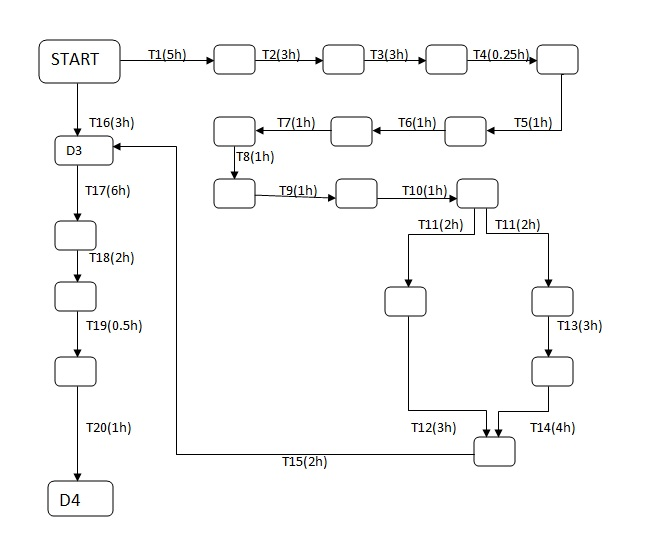
\includegraphics[scale=0.7]{img/PERT.jpg}
Present the schedules on which performance and resource planning are
based. Include a task table, Gantt and PERT charts.

%%%%%%%%%%%%%%%%%%%%%%%%%%%%%%%%%%%%%%%%%%%%%%%%%%%%%%%%%%%%%%%%%%%%%%%%%%%%%%

\subsection{Equipment, Materials, Facilities, and Other Resources}

%%%%%%%%%%%%%%%%%%%%%%%%%%%%%%%%%%%%%%%%%%%%%%%%%%%%%%%%%%%%%%%%%%%%%%%%%%%%%%

\section{Assurance Plan}


The Quality Assurance Plan( The QAP) is the basis for maintaining the quality of our product on the highest level that matches the requirements of the given software system. The QAP will be overseen by the team to maintain quality improvement activities, such as monitoring, adding features and evaluating defects. The purpose of the QAP is designed to match the following requirements:\\

\begin{itemize}
\item to perform suitable actions when possibilities for improvements in service are identified.\\
\item to implement corrective action when technical issues or bugs are found.\\
\item To ensure that the software system is maintaining properly all the time.\\
\end{itemize}

Our team will mainly rely on Risk Management Plan and Product Requirements Specification to keep the product quality to the appropriate level.\\

Team activities:\\

Prior to making any changes to code, it will be reviewed by the team and will be submitted to GitHub, supporting version control of source code. After altering any part of the code, we invoke test sets to check if the corresponding oracles match expected outputs. Apart from that, we use black box testing with other teams to check if they can find bugs, as they have a fresh look to the product.\\

This documentation does not contain any details regarding the action taken.\\


Describe the activities to be performed by for assurance of the
software and other deliverables.

Assurance activities include:
\begin{enumerate}
\item Review and acceptance testing of products
\item Verification and validation procedures
\end{enumerate}

The contents of this subsection will be explained later in the 1st
semester in the PSD lectures. For initial hand-in deadline, you may
leave this subsection blank or make your best effort to produce an
assurance plan.

%%%%%%%%%%%%%%%%%%%%%%%%%%%%%%%%%%%%%%%%%%%%%%%%%%%%%%%%%%%%%%%%%%%%%%%%%%%%%%

\section{Risk Management Plan}

Here is the list of risk tables
\begin{PSDRisk}{1}{}
  \PSDRiskID{1}%
  \PSDTaskOutcomes{Requirements Specification}%
  \PSDTaskDeliverables{D3}%
  \PSDTaskRisks{}
\end{PSDTask}

%https://github.com/Stringsy/psd3-groupwork/wiki/_pages

%%%%%%%%%%%%%%%%%%%%%%%%%%%%%%%%%%%%%%%%%%%%%%%%%%%%%%%%%%%%%%%%%%%%%%%%%%%%%%

\section{Configuration Management Plan}

Describe the activities and plans for configuration management to be
performed by the organization preparing this Management Plan. The
primary topics for the plan include:

\begin{enumerate}
\item Configuration management process
\item Configuration control activities
\item Configuration identification
\item Configuration change control
\end{enumerate}

The contents of this subsection will be explained later in the 1st
semester in the PSD lectures. For initial hand-in deadline, you may
leave this subsection blank or make your best effort to produce an
assurance plan.

%%%%%%%%%%%%%%%%%%%%%%%%%%%%%%%%%%%%%%%%%%%%%%%%%%%%%%%%%%%%%%%%%%%%%%%%%%%%%%

\appendix

\section{Glossary}

\textbf{PSD3:} Professional Software Development 3\\

Including expansions of non-standard abbreviations and acronyms and
other key definitions.  You may find it useful to maintain a glossary
as a shared section amongst all your PSD documents. using the
\verb!\input{}! macro.

\end{document}

%%%%%%%%%%%%%%%%%%%%%%%%%%%%%%%%%%%%%%%%%%%%%%%%%%%%%%%%%%%%%%%%%%%%%%%%%%%%%%

